% !TEX root = sbaconf.tex
%===============================================================================
% $Id: ifacconf.tex 19 2011-10-27 09:32:13Z jpuente $  
% Template for IFAC meeting papers
% Copyright (c) 2007-2008 International Federation of Automatic Control
%===============================================================================
\documentclass[a4paper]{ifacconf}

\usepackage{graphicx,amsmath,url}      % include this line if your document contains figures
\usepackage[round]{natbib}             % required for bibliography
%===============================================================================

% If in Portuguese or Spanish, choose
\def\portugues{1} 
\usepackage[spanish,brazil,english]{babel}
\usepackage[T1]{fontenc}
\usepackage[utf8]{inputenc}
\usepackage{unicode}
\usepackage{ae}
\usepackage{placeins}
\usepackage{multicol}
\usepackage{cuted}
\usepackage{amsmath} % for 'bmatrix' environment


\if\portugues1
% =====================================================================
% =====================================================================
% If the manuscript is in Spanish, please change the texts adequatelly.
% You may also add other definitions in this part.
 \newtheorem{teorema}[thm]{{\em Teorema}}{ }
 \newtheorem{lema}[thm]{{\em Lema}}{ }
 \newtheorem{corolario}[thm]{{\em Corolário}}{ }
 \newenvironment{prova}{{\bf Prova.}}{ }
% ===============================================================
\fi

\begin{document}
	
    \selectlanguage{brazil}
	
    \begin{frontmatter}
        
        \title{Trabalho computacional \\Teoria de Sistemas Lineares \\Síntese de observador e controlador por realimentação de estados para controle de suspensão veicular ativa, não-linear} 

        \author[First]{Charles Quirino Pimenta} 
        
        \address[First]{Programa de Pós-Graduação em Engenharia Elétrica - Universidade Federal de 
Minas Gerais - Av. Antônio Carlos 6627, 31270-901, Belo Horizonte, MG, Brasil\\ e-mail:charlesqp@ufmg.br.}
        
        \selectlanguage{english}
        \renewcommand{\abstractname}{{\bf Abstract:~}}
        \begin{abstract} Colocar o abstract em ingles aqui
        
        \vskip 1mm% não altere esse espaçamento
        \selectlanguage{brazil}
        {\noindent \bf Resumo}:Colocar o abstract em português aqui
        \end{abstract}
        
        \selectlanguage{english}
        
        \begin{keyword} Colocar palavres chave em ingles aqui 
        
        \vskip 1mm% não altere esse espaçamento
        \selectlanguage{brazil}
        {\noindent\it Palavras-chaves:} Colocar palavres chave em português aqui 
        \end{keyword}
        
        \selectlanguage{brazil}
        
        \end{frontmatter}

    \section{Introdução}
    Em sistemas veiculares automotores é necessário controlar as vibrações de sistemas mecânicos com a finalidade de minimizar as vibrações transmitidas ao chassi do veículo e proporcionar maior conforto aos seus utilizadores.
    Em veículos é necessário realizar o controle de vibrações transmitidas pela pista, uma vez que estas causam desconforto aos passageiros e diminuem o contato entre pneu e pista, e diminuem a estabilidade do veículo.
    Existem três tipos de suspensão veicular: suspensão passiva, ativa e semiativa. Esta classificação é dada de acordo com a presença e o tipo de controle utilizado para minimizar as vibrações transmitidas ao chassi.
    Sistemas de controle passivo são os sistemas de suspensão convencionais, são compostos por molas, amortecedores e pneus. O sistema de controle passivo só é capaz de atuar em uma banda de frequência restrita, limitando-se a utilização em sistemas com frequências fora desta banda. Este sistema proporciona uma viagem menos confortável e estável ao carro em comparação aos sistemas de amortecimento ativo e semiativo.
    Um sistema de suspensão ativa é um sistema capaz de atuar em diferentes bandas de frequência, através da utilização de atuadores, sensores e sistemas eletrônicos de controle. A sua desvantagem está na elevada quantidade de energia que os componentes utilizados necessitam, necessitando do uso de uma fonte de energia externa, isto implica em um produto final de custo mais elevado quando comparado com sistemas de suspensão passiva.
    Um sistema de suspensão semiativa também apresenta funcionalidade em diversas bandas de frequência e não possui a obrigatoriedade de uma fonte de tensão externa permanente de grande porte. Outra vantagem deste tipo de sistema é que este, na falta de energia, comporta-se como um sistema passivo, agregando mais confiabilidade e segurança ao veículo. Por fim, um sistema de suspensão semiativa possui custo intermediário entre as demais opções.
    Neste trabalho, focou-se sobre o sistema de suspensão ativa com um atuador generalizado. Este trabalho apresentará a implementação de um controlador ativo aplicado a um sistema de suspensão veicular com modelo não linearizado.
    \section{Objetivos}
    Projetar e analisar um observador e um controlador por realimentação no espaço de estados para o modelo linearizado de um sistema de suspensão veicular ativa, não-linear, através do controle da amplitude da aceleração e deslocamento vertical aos quais os passageiros estão submetidos. 
    
    Para alcançar o objetivo principal, os seguintes objetivos específicos foram propostos:
    \begin{itemize}
        \item Realizar a modelagem matemática de um sistema de suspensão não linear de um quarto de veículo com dois graus de liberdade
        \item Realizar a linearização do modelo completo proposto
        \item Projetar um observador de estados para a estimação das variáveis de estados necessárias para o funcionamento da estratégia de controle.
        \item Projetar um controlador de forma a aumentar o nível de conforto e/ou dirigibilidade do veículo
        \item Realizar simulações temporais com o controlador proposto para o sistema linearizado e original.
    \end{itemize}
    \section{Revisão Bibliográfica}
    \subsection{Modelo matemático do sistema de suspensão não linear para um quarto de veículo }
    O modelo de um quarto de carro consiste em isolar uma quarta parte do veiculo e estudar isoladamente o comportamento do sistema de suspensão para esta seção. Para veículos com peso igualmente distribuído, os resultados são muito próximos ao do modelo completo. Geralmente os modelos para um quarto de carro tem 2 graus de liberdade, sendo estes o deslocamento vertical da massa suspensa e da massa não suspensa. Este modelo pode ser observado na figura \ref{fig:massa_mola_nao_linear_controlavel} a seguir. Este modelo é composto por uma massa suspensa que representa a carroceria do veiculo e uma massa não suspensa que representa o conjunto eixo e roda. Estas massas são conectadas pela mola e pelo amortecedor. O contato do veiculo com a pista de rolamento é realizado através do pneu. O sistema é exitado, ou perturbado, pelas irregularidades da pista.
    \FloatBarrier
    \begin{figure}[htbp]
        \begin{centering}
            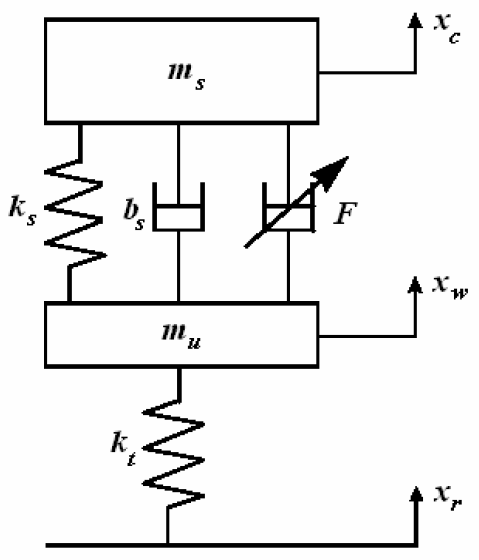
\includegraphics[width=5cm]{img/massa_mola_nao_linear_controlavel.png}
            \caption{Modelo de suspensão para um quarto de carro.} 
            \label{fig:massa_mola_nao_linear_controlavel}
        \end{centering}
    \end{figure}
    \FloatBarrier
    Na figura \ref{fig:massa_mola_nao_linear_controlavel} temos que $m_s$ representa a massa suspensa que consiste em um quarto da massa total da carroceria do veiculo em \emph{kg}, $m_u$ representa a massa não suspensa ou a massa do eixo e da roda em \emph{kg}, $b_s$ representa o o coeficiente de amortecimento do amortecedor passivo em \emph{Ns/m}, $k_s$ representa o coeficiente de elasticidade do feixe de molas da suspensão, segundo a lei de hooke, em \emph{N/m}, $k_t$ representa o coeficiente de elasticidade do pneu, segundo a lei de hooke, em \emph{N/m}, $x_r$ representa o deslocamento vertical da pista, onde o sufixo $r$ significa \emph{road}, em \emph{m}, $x_w$ representa o deslocamento vertical da roda, onde o sufixo $w$ significa \emph{wheel}, em \emph{m} e $x_c$ representa o deslocamento vertical da carroceria, onde o sufixo $c$ significa \emph{carr}, em \emph{m}. Na mesma figura o simbolo $F$ representa a atuação de um dispositivo amortecedor com características dinâmicas, seja ele ativo ou semi-ativo, em \emph{N}.
    
    O diagrama de corpo livre do sistema pode ser construído tomando-se como referencia a coordenada da posição do eixo da roda $x_w$ como pode ser observado nas figuras \ref{fig:corpo_livre_ms} e \ref{fig:corpo_livre_mu} a seguir:
    \FloatBarrier
    \begin{figure}[htbp]
        \begin{centering}
            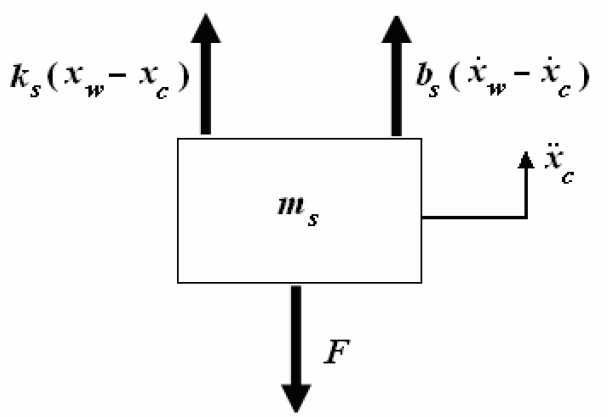
\includegraphics[width=5cm]{img/corpo_livre_ms.png}
            \caption{Diagrama de corpo livre para a massa $m_s$.} 
            \label{fig:corpo_livre_ms}
        \end{centering}
    \end{figure}
    \FloatBarrier
    \begin{figure}[htbp]
        \begin{centering}
            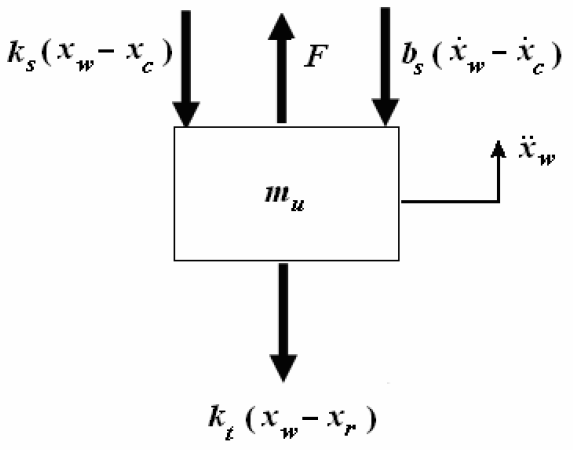
\includegraphics[width=5cm]{img/corpo_livre_mu.png}
            \caption{Diagrama de corpo livre para a massa $m_u$.} 
            \label{fig:corpo_livre_mu}
        \end{centering}
    \end{figure}
    \FloatBarrier
    
    Aplicando a segunda lei de Newton $\sum{F}=m.a$, a cada uma das massas separadamente, o sistema para o modelo de um quarto de carro da figura \ref{fig:massa_mola_nao_linear_controlavel} pode ser representado pela seguinte equação:
    
    \begin{equation} \label{eq:massa_mola_linear}
    \begin{split}
        m_{s} \ddot{x}_{c} =&  b_{s}(\dot{x}_{w}-\dot{x}_{c}) + k_{s}(x_{w}-x_{c}) - F\ \\
        m_{u} \ddot{x}_{w} =& -b_{s}(\dot{x}_{w}-\dot{x}_{c}) - k_{s}(x_{w}-x_{c})  k_{t}(x_{w}-x_{r}) + F
    \end{split}
    \end{equation}
    
    A equação \ref{eq:massa_mola_linear} representa o modelo do sistema na forma linear. Porém a mola $k_s$, o amortecedor $b_s$ e o amortecedor dinâmico ativo podem ser modelados através de modelos lineares ou modelos não lineares. \\
    Uma mola linear obedece a lei de Hooke apresentando uma deformação proporcional ao carregamento. Em uma mola não linear o coeficiente de elasticidade da mola cresce exponencialmente conforme se afasta do ponto de equilíbrio estático.
    Para um modelo de mola não linear, podemos utilizar seguinte expressão para a força da mola $ k_{s}(x_{w}-x_{c})$:
    
    \begin{equation} \label{eq:mola_nao_linear}
        k_{s}(x_{w}-x_{c}) = k^{l}_{s}(x_{w}-x_{c})+k^{nl}_{s}(x_{w}-x_{c})^{3}
    \end{equation}
        
    Na equação \ref{eq:mola_nao_linear} o coeficiente $k^{l}_{s}$ representa o coeficiente de elasticidade do termo da faixa de operação linear e o coeficiente $k^{nl}_{s}$] representa o coeficiente de elasticidade do termo da faixa de operação não linear do feixe de molas em uma situação real.\\
    A não linearidade do amortecedor permite que pequenos movimentos causados pelo perfil da estrada gerem apenas um pequeno impacto na carroceria além de apresentar saturação e histerese. Para um modelo de amortecedor não linear, podemos utilizar a seguinte expressão:
 
    \begin{equation} \label{eq:amortecedor_nao_linear}
        \begin{aligned}
        b_{s}(\dot{x}_{w}-\dot{x}_{c}) =\ \ &b^{l}_{s}(\dot{x}_{w}-\dot{x}_{c}) - b^{y}_{s}\mid\dot{x}_{w}-\dot{x}_{c}\mid \\
        + &b^{nl}_{s}\sqrt{\mid\dot{x}_{w}-\dot{x}_{c}\mid}sgn(\dot{x}_{w}-\dot{x}_{c})  
        \end{aligned}
    \end{equation}
    
    Na equação \ref{eq:amortecedor_nao_linear} o coeficiente $b^{l}_{s}$ representa o coeficiente de amortecimento do termo da faixa de operação linear, o coeficiente $b^{l}_{s}$ representa o coeficiente de amortecimento do termo da faixa de operação não linear e o coeficiente $b^{y}_{s}$ representa a característica de comportamento assimétrico do amortecedor.
    
    Substituindo as equações \ref{eq:mola_nao_linear} e \ref{eq:amortecedor_nao_linear} em \ref{eq:massa_mola_linear} obtemos as seguintes equações diferenciais dinâmicas de segunda ordem que representam a dinâmica de um sistema de suspensão ativa não linear:
    
    \begin{equation} \label{eq:massa_mola_nao_linear}
        \begin{aligned}
         m_{s} \ddot{x}_{c} =\ \ &k^{l}_{s}(x_{w}-x_{c})+k^{nl}_{s}(x_{w}-x_{c})^{3}+b^{l}_{s}(\dot{x}_{w}-\dot{x}_{c})\\
                            -&b^{y}_{s}\mid\dot{x}_{w}-\dot{x}_{c}\mid+b^{nl}_{s}\sqrt{\mid\dot{x}_{w}-\dot{x}_{c}\mid}sgn(\dot{x}_{w}-\dot{x}_{c})\\ 
                            -&F\\
         m_{u} \ddot{x}_{w} = -&k^{l}_{s}(x_{w}-x_{c})-k^{nl}_{s}(x_{w}-x_{c})^{3}-b^{l}_{s}(\dot{x}_{w}-\dot{x}_{c})\\  
                            +&b^{y}_{s}\mid\dot{x}_{w}-\dot{x}_{c}\mid-b^{nl}_{s}\sqrt{\mid\dot{x}_{w}-\dot{x}_{c}\mid}sgn(\dot{x}_{w}-\dot{x}_{c})\\
                            -&k_{t}(x_{w}-x_{r})+F\\
        \end{aligned}
    \end{equation}
    \subsection{Modelo Linearizado de um sistema de suspensão semi-ativa, não linear, de um quarto de veículo, com dois graus de liberdade }
    Realizando a distributiva no sistema descrito em \ref{eq:massa_mola_nao_linear} e Propondo as seguintes substituições para as variáveis de estado das equações e reorganizando os termos, obtemos: 
    \begin{equation*}
        \begin{split}
            x_{1}=&x_{c};\ \ \\
            x_{2}=&\dot{x}_{c};\ \ \\
            x_{3}=&x_{w};\ \ \\
            x_{4}=&\dot{x}_{w};\ \ \\
        \end{split}
        \begin{split}
            \dot{x}_{1}=&\dot{x}_{c};\ \ \\
            \dot{x}_{2}=&\ddot{x}_{c};\ \ \\
            \dot{x}_{3}=&\dot{x}_{w};\ \ \\
            \dot{x}_{4}=&\ddot{x}_{w};\ \ \\
        \end{split}
        \begin{split}
            w=&x_{r};\ \ \\
            u=&F;\ \ \\
        \end{split} 
    \end{equation*}
    \begin{equation} \label{eq:massa_mola_nao_linear}
        \begin{aligned}
        \dot{x}_{1}=&\ \ \ \ x_{2}\\
        \dot{x}_{2}=&-\frac{k^l_s}{m_s}x_1-\frac{b^l_s}{m_s}x_2+\frac{k^l_s}{m_s}x_3+\frac{b^l_s}{m_s}x_4-\frac{k^{nl}_s}{m_s}(x_3-x_1)^3\\
                    &+\frac{b^y_s}{m_s}\mid x_4-x_2\mid+\frac{b^{nl}_s}{m_s}\sqrt{\mid x_4-x_2\mid}sgn(x_4-x_2)\\
                    &-\frac{1}{m_s}u\\
        \dot{x}_{3}=&\ \ \ \ x_{4}\\
        \dot{x}_{4}=&\ \ \ \ \frac{k^l_s}{m_u}x_1+\frac{b^l_s}{m_u}x_2-\frac{k^l_s}{m_u}x_3-\frac{b^l_s}{m_u}x_4+\frac{k^{nl}_s}{m_u}(x_3-x_1)^3\\
                    &-\frac{b^y_s}{m_u}\mid x_4-x_2\mid-\frac{b^{nl}_s}{m_u}\sqrt{\mid x_4-x_2\mid}sgn(x_4-x_2)\\
                    &+\frac{k_t}{m_u}w+\frac{1}{m_u}u\\
        \end{aligned}
    \end{equation}
    
    \section{Metodologia}
    \subsection{Linearização do modelo em espaço de estados}
        
    O sistema proposto possui um ponto de equilíbrio na origem do sistema:
    \begin{equation*}
        \begin{split}
        x_1=\ \ &0\\
        x_2=\ \ &0\\
        x_3=\ \ &0\\
        x_4=\ \ &0\\
        \end{split}
    \end{equation*}
    Calculamos a Jacobiana do Sistema para realizar a linearização em torno do ponto de operação escolhido:
    
    \begin{equation} \label{eq:Jacobian_A}
    \mathbf{J_A}(x_1,x_2,x_3,x_4) =
        \begin{bmatrix}
            \frac{\partial x_1}{\partial x_1} & 
            \frac{\partial x_1}{\partial x_2} & 
            \frac{\partial x_1}{\partial x_3} &
            \frac{\partial x_1}{\partial x_4} &\\[1ex] % <-- 1ex more space between rows of matrix
            \frac{\partial x_2}{\partial x_1} & 
            \frac{\partial x_2}{\partial x_2} & 
            \frac{\partial x_2}{\partial x_3} &
            \frac{\partial x_2}{\partial x_4} &\\[1ex]
            \frac{\partial x_3}{\partial x_1} & 
            \frac{\partial x_3}{\partial x_2} & 
            \frac{\partial x_3}{\partial x_3} &
            \frac{\partial x_3}{\partial x_4} &\\[1ex]
            \frac{\partial x_4}{\partial x_1} & 
            \frac{\partial x_4}{\partial x_2} & 
            \frac{\partial x_4}{\partial x_3} &
            \frac{\partial x_4}{\partial x_4} &\\[1ex]
    \end{bmatrix}
    \end{equation}
    
    \begin{equation} \label{eq:eval_A}
        \mathbf{A=J_A} \Bigr\rvert_{(x_1=0;x_2=0;x_3=0;x_4=0)} \\
    \end{equation}
    
    \begin{equation} \label{eq:Jacobian_B}
    \mathbf{J_B}(w,F) =
        \begin{bmatrix}
            \frac{\partial x_1}{\partial w} & 
            \frac{\partial x_1}{\partial F} &\\[1ex] % <-- 1ex more space between rows of matrix
            \frac{\partial x_2}{\partial w} & 
            \frac{\partial x_2}{\partial F} &\\[1ex]
            \frac{\partial x_3}{\partial w} & 
            \frac{\partial x_3}{\partial F} &\\[1ex]
            \frac{\partial x_4}{\partial w} & 
            \frac{\partial x_4}{\partial F} &\\[1ex]
    \end{bmatrix}
    \end{equation}
    
    \begin{equation} \label{eq:eval_B}
        \mathbf{B=J_B} \Bigr\rvert_{(w;F)} \\
    \end{equation}
    
    Aplicando o sistema de equações dinâmicas não lineares descrito em \ref{eq:massa_mola_nao_linear} nas equações \ref{eq:Jacobian_A}, \ref{eq:Jacobian_B}, \ref{eq:eval_A}, \ref{eq:eval_B} obteremos as matrizes A e B do sistema linearizado exibidas a seguir:
    
    
    \begin{equation*} 
    \begin{split}
        \mathbf{A} =
        \begin{bmatrix}
            0 & 1 & 0 & 0 & \\
            -\frac{k_{s}^{l}}{m_s}&-\frac{b_{s}^{l}}{m_s}&\frac{k_{s}^{l}}{m_s}&\frac{b_{s}^{l}}{m_s} &\\ \\
            0 & 0 & 0 & 1 & \\
            \frac{k_{s}^{l}}{m_u}&\frac{b_{s}^{l}}{m_u}&-\frac{(k_{s}^{l}+k_t)}{m_u}&-\frac{b_{s}^{l}}{m_u} &\\
        \end{bmatrix};
    \end{split}
    \begin{split}
       \mathbf{x} = 
        \begin{bmatrix}
             x_1 &\\
             x_2 &\\
             x_3 &\\
             x_4 &\\
        \end{bmatrix}; 
    \end{split}
    \end{equation*}
    
    \begin{equation} 
    \begin{split}
        \mathbf{B} = 
        \begin{bmatrix}
            0 & 0 & \\
            0 & -\frac{1}{m_s}&\\ \\
            0 & 0 & \\
            \frac{k_t}{m_u}&\frac{1}{m_u} \\
        \end{bmatrix}
    \end{split}
    \end{equation}
    
    É esperado que o  sistema linearizado se aproxime do sistema não linear enquanto opere na vizinhança do ponto de equilíbrio utilizado para linearização. Que para este caso é a origem do sistema formado pelas variáveis de estado.
    \subsection{Simulação da resposta temporal do modelo linearizado}
    Abaixo seguem figuras que ilustram a simulação temporal do sistema não linear e linearizado para 3 diferentes condições iniciais a parâmetros do sistema dados a seguir: 
    
    \begin{equation*} 
    \begin{split}
        \begin{bmatrix}
            x_c & \dot{x}_c & x_w & \dot{x}_w & \\
        \end{bmatrix}=
    \end{split}
    \begin{split}
        \begin{bmatrix}
            -0.01& -0.01& 0& 0& \\
             -0.1&  -0.1& 0& 0& \\
             -0.5&  -0.5& 0& 0&\\
        \end{bmatrix}
    \end{split}
    \end{equation*}
    
   \begin{equation} \label{eq:parametros}
        \begin{split} 
        m_s =   & 290     [kg]\\
        m_u =   & 40      [kg]\\
        b^{l}_s =  & 700  [Ns.m^{-1}]\\
        b^{nl}_s =  & 200      [Ns.m^{-1}]\\
        b^{y}_s=  & 400      [Ns.m^{-1}]\\
        k^{l}_s =  & 235.10^2 [N.m^{-1}]\\
        k^{nl}_s = & 235.10^4 [N.m^{-1}]\\
        k_t =  & 190.10^3 [N.m^{-1}]\\
        \end{split}
    \end{equation}

    \FloatBarrier
    \begin{figure}[htbp]
        \begin{centering}
            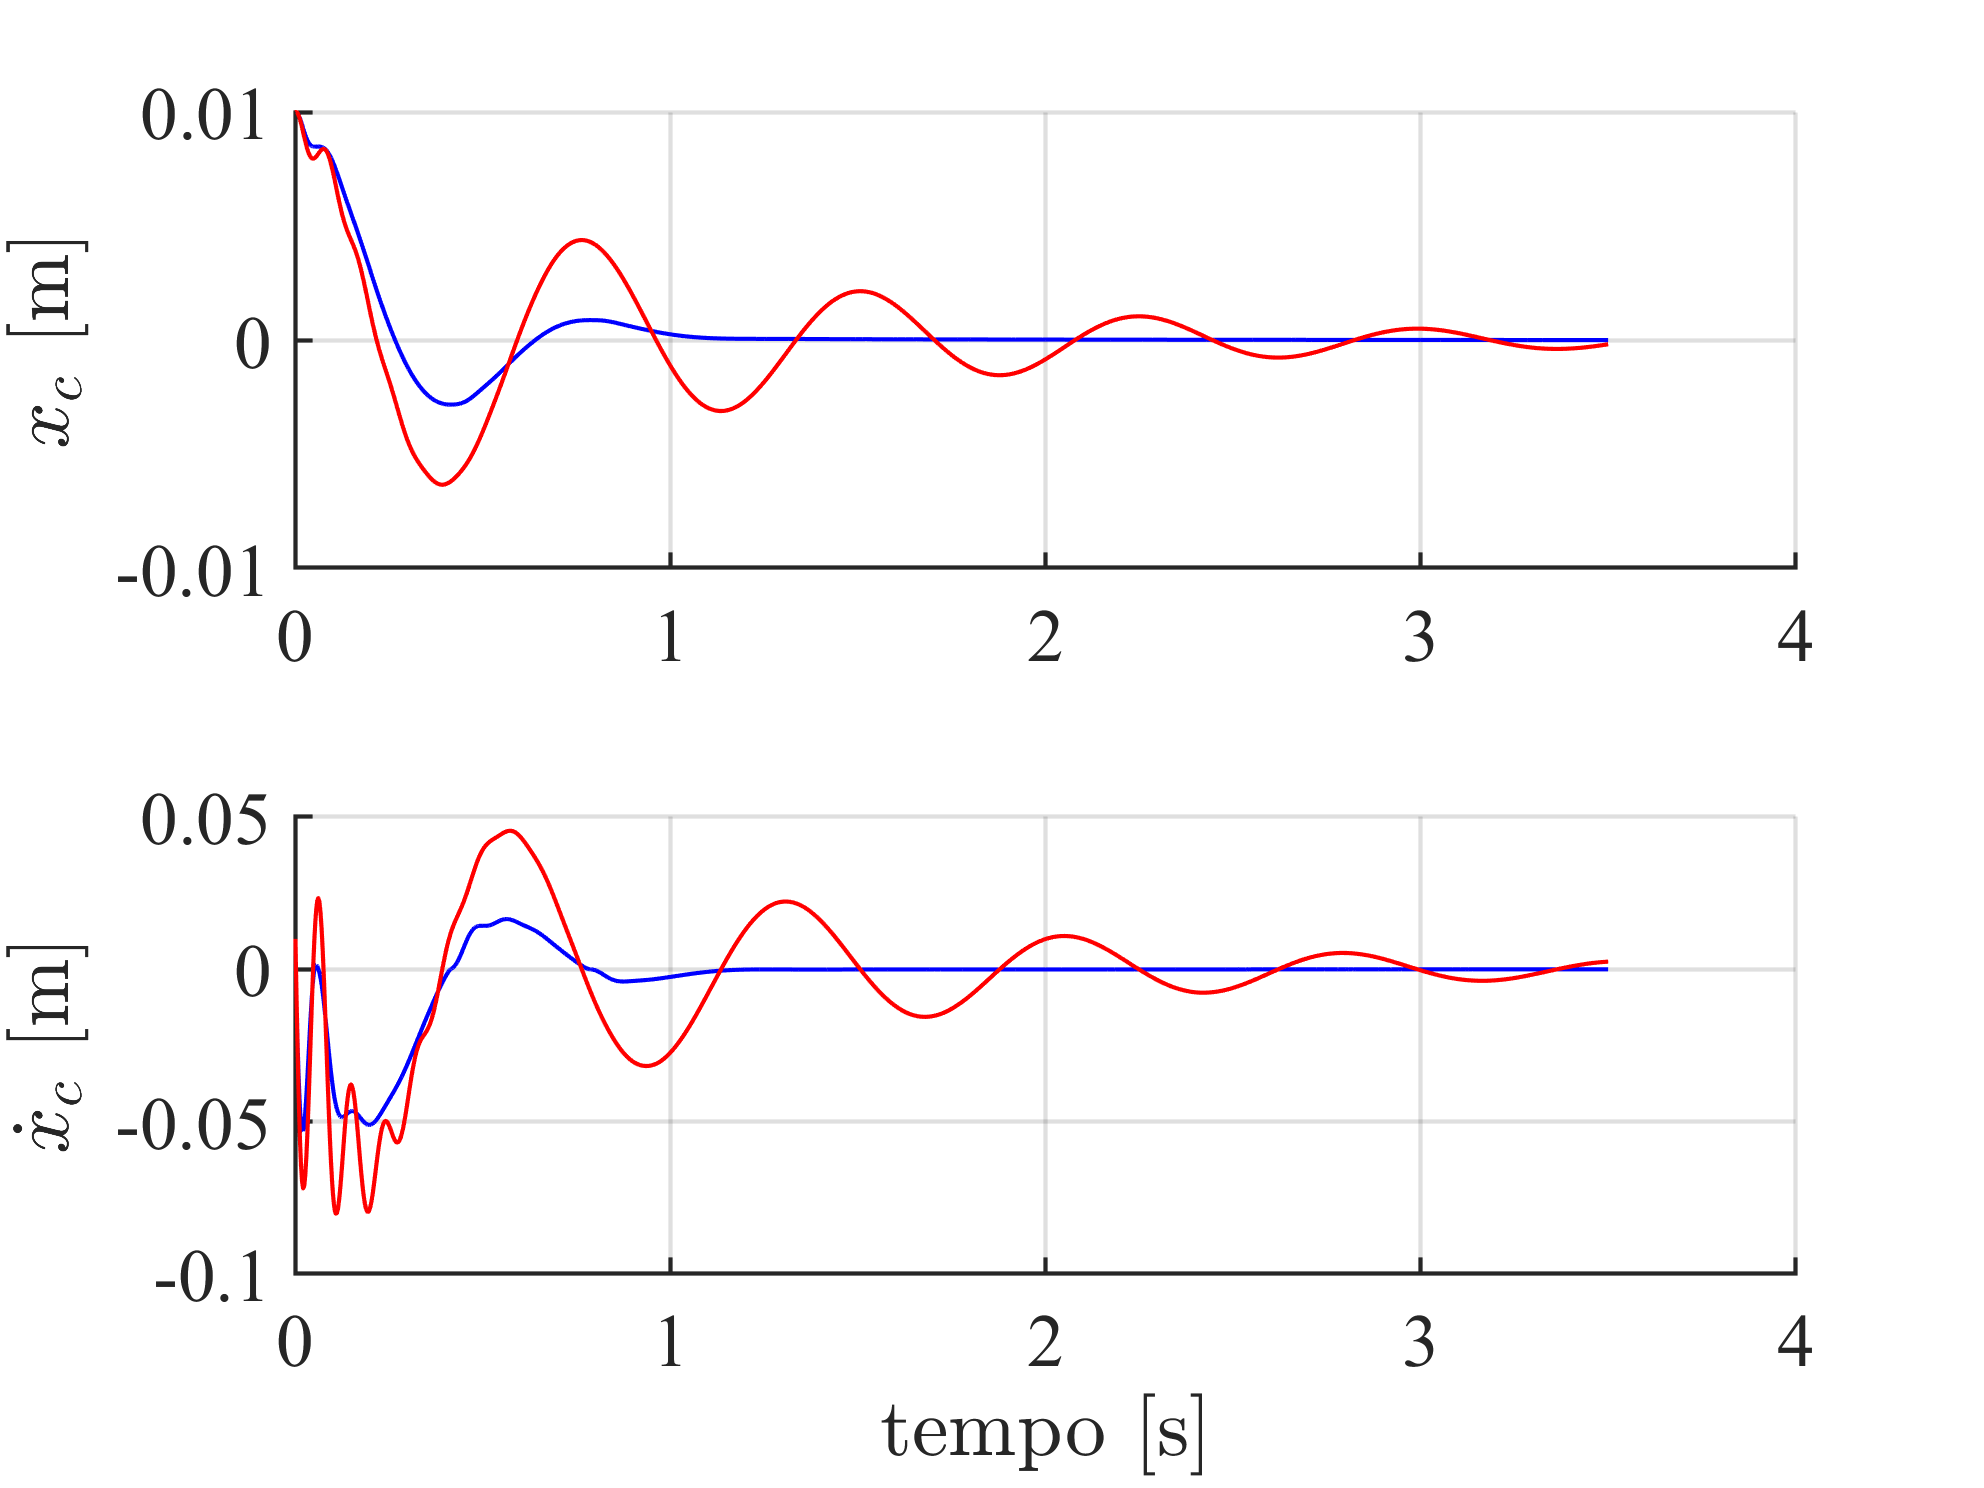
\includegraphics[width=7cm]{img/sim_temp_xc_n001_dxc_n001.png}
            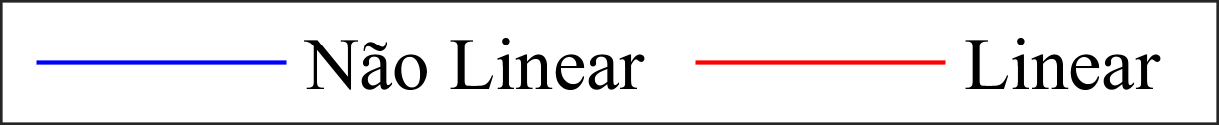
\includegraphics[width=5cm]{img/sim_temp_Leg.png}
            \caption{Simulação temporal do sistema para as condições iniciais:  $[x_c, \dot{x}_c, x_w, \dot{x}_w]=[-0.01,-0.01,0,0]$}
            \label{fig:sim_temp_xc_n01_dxc_n01}
        \end{centering}
    \end{figure}
    \FloatBarrier
    
    \FloatBarrier
    \begin{figure}[htbp]
        \begin{centering}
            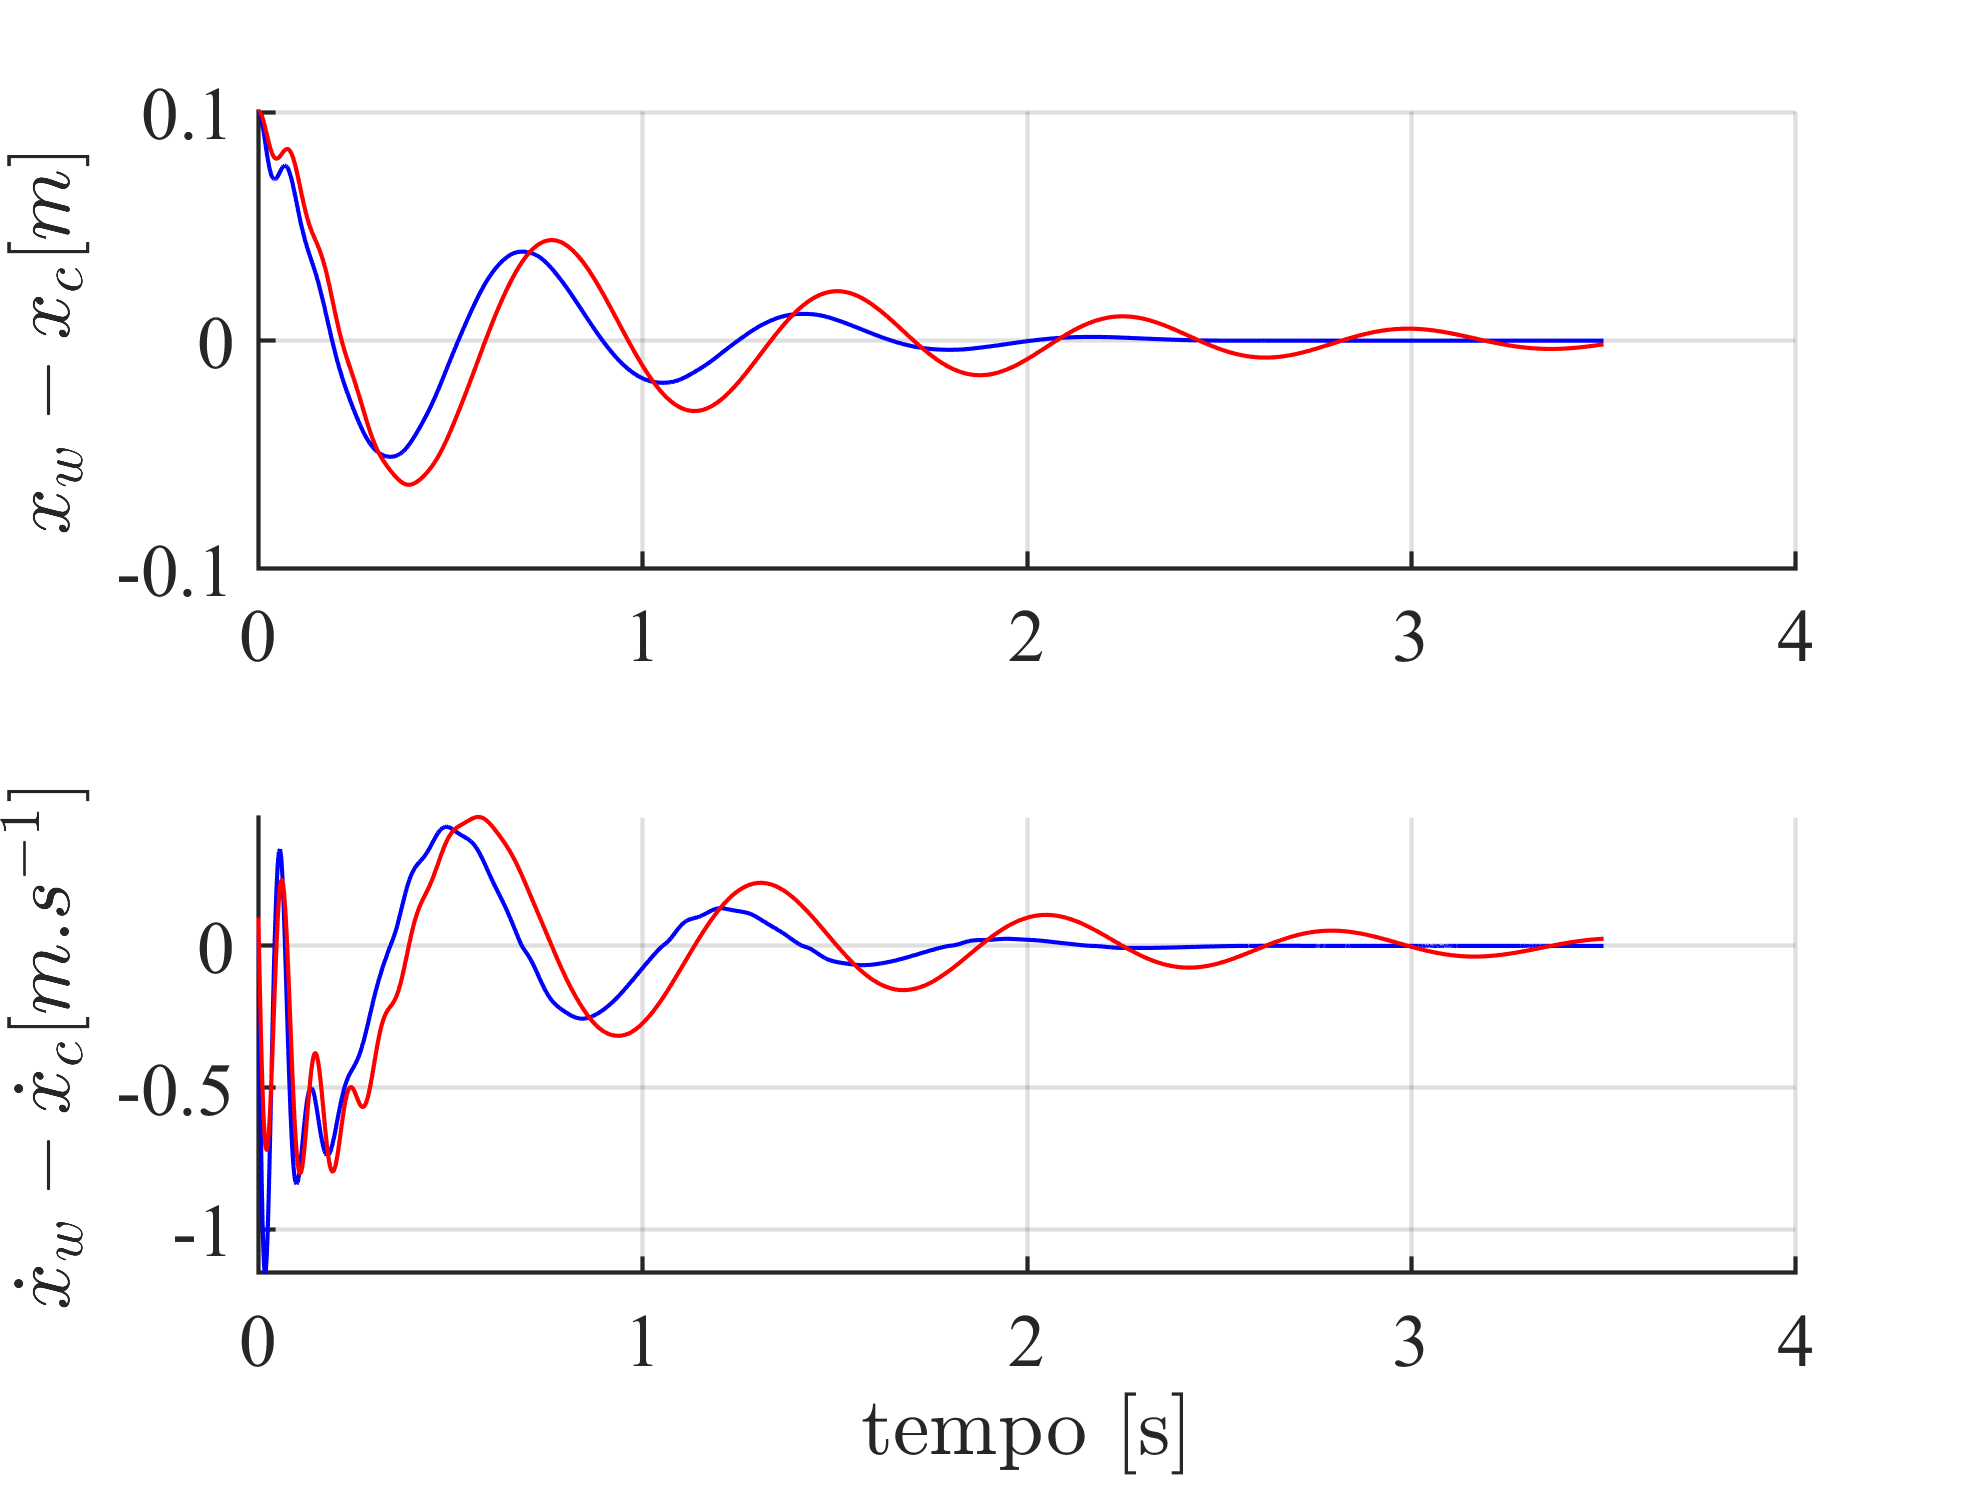
\includegraphics[width=7cm]{img/sim_temp_xc_n01_dxc_n01.png}
            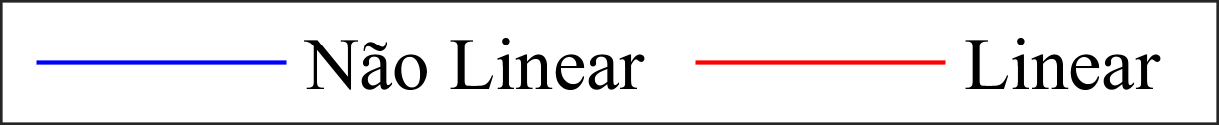
\includegraphics[width=5cm]{img/sim_temp_Leg.png}
            \caption{Simulação temporal do sistema para as condições iniciais:  $[x_c, \dot{x}_c, x_w, \dot{x}_w]=[-0.1,-0.1,0,0]$}
            \label{fig:sim_temp_xc_n01_dxc_n01}
        \end{centering}
    \end{figure}
    \FloatBarrier
    
    \FloatBarrier
    \begin{figure}[htbp]
        \begin{centering}
            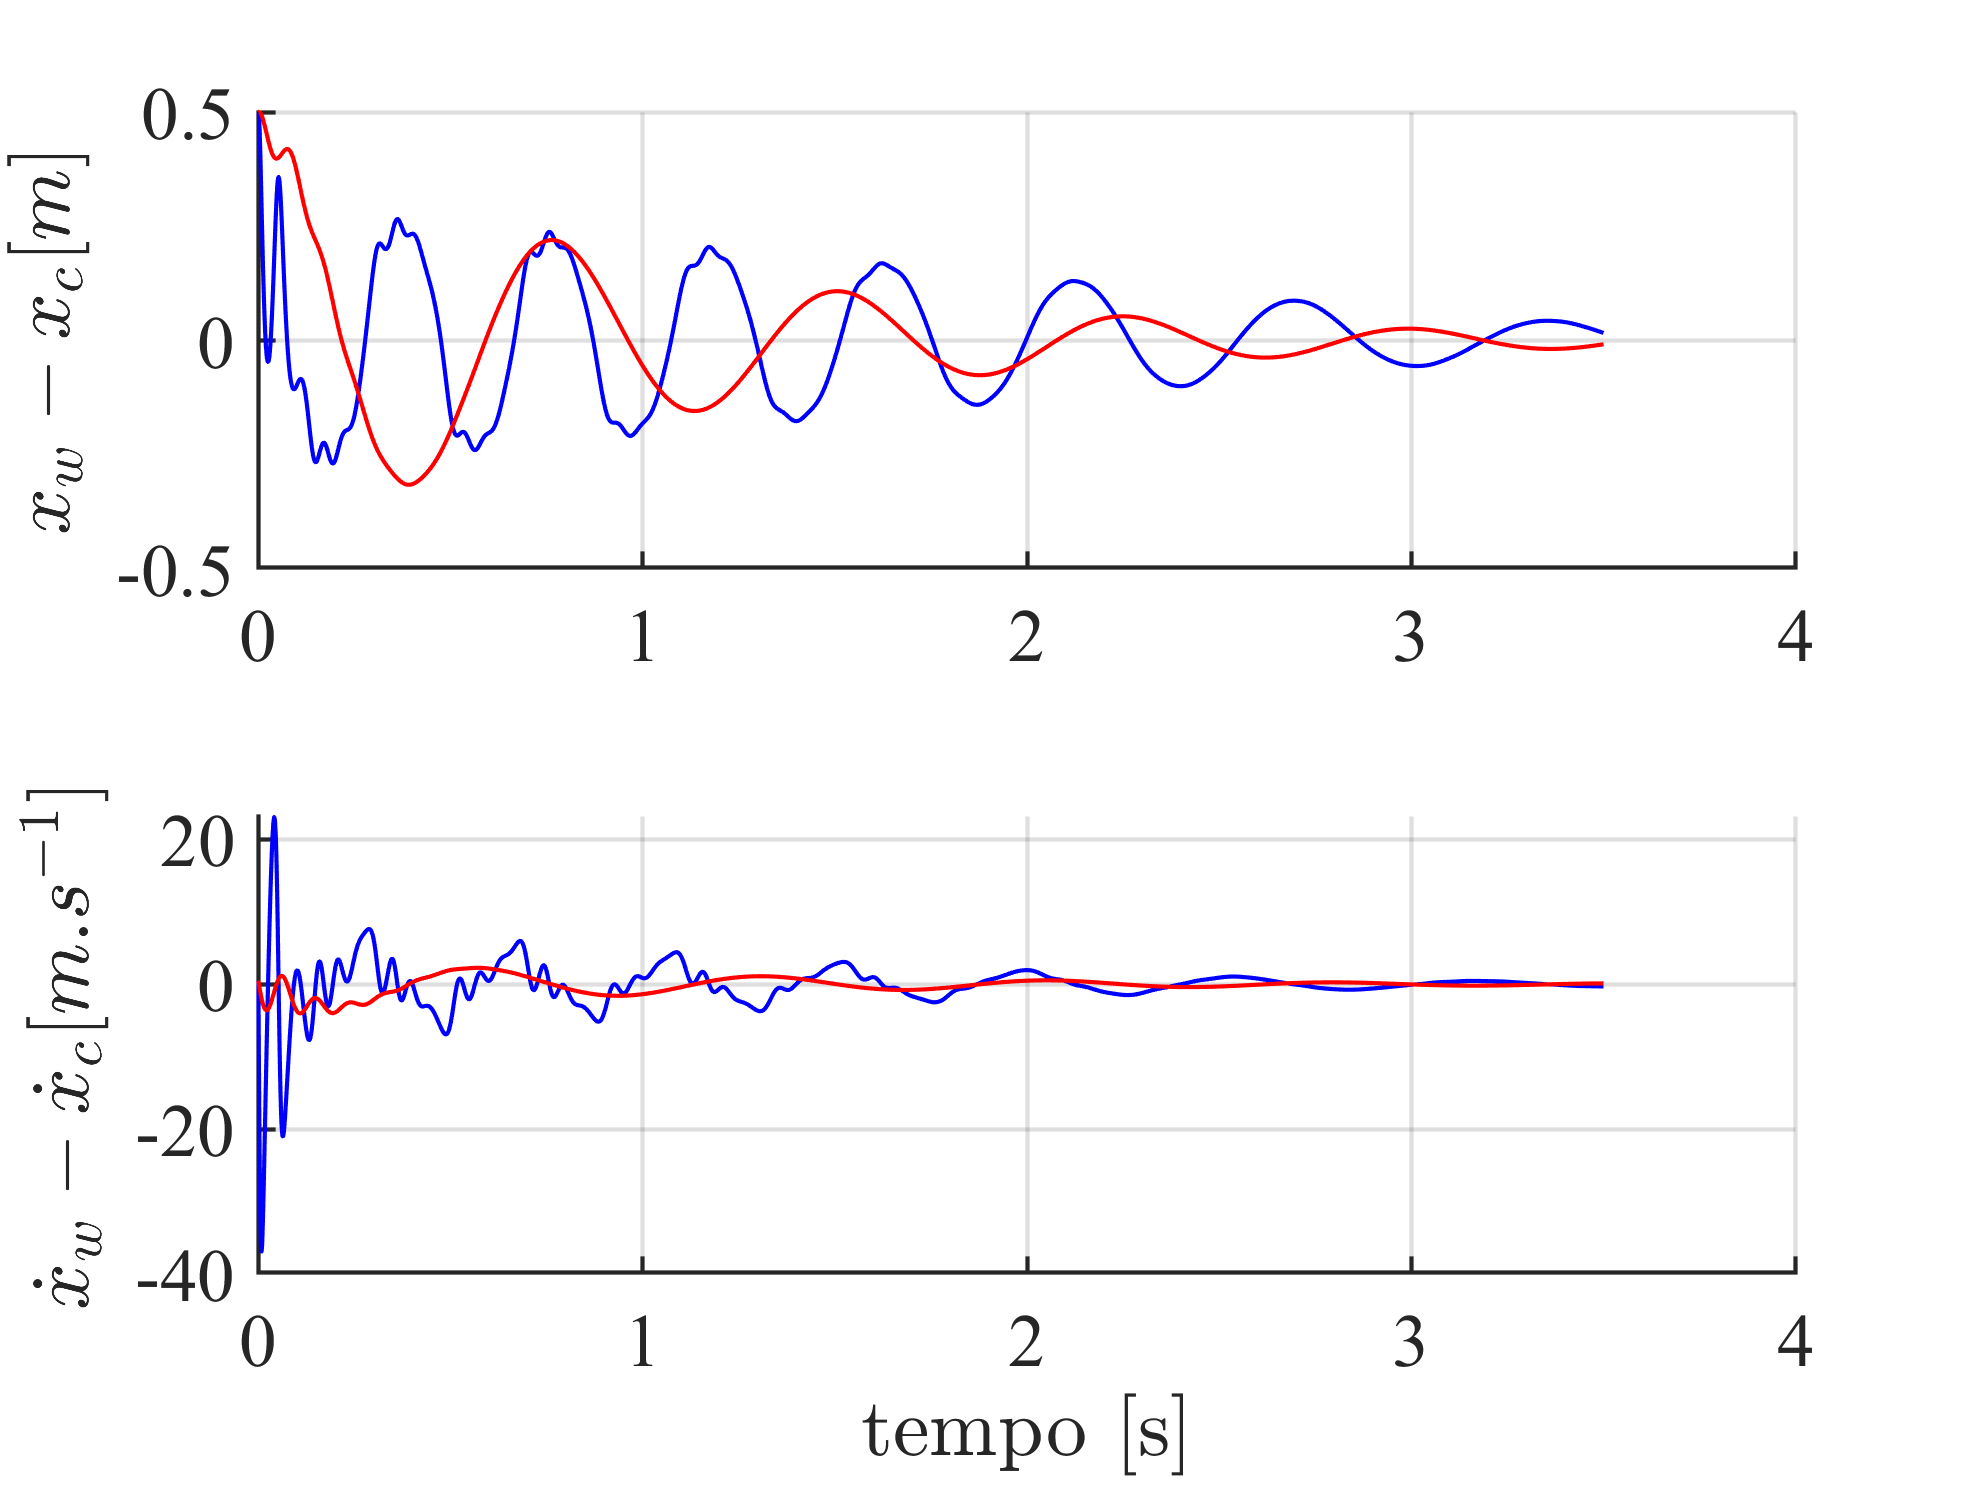
\includegraphics[width=7cm]{img/sim_temp_xc_n05_dxc_n05.png}
            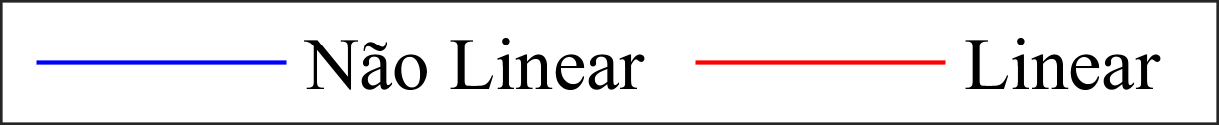
\includegraphics[width=5cm]{img/sim_temp_Leg.png}
            \caption{Simulação temporal do sistema para as condições iniciais:  $[x_c, \dot{x}_c, x_w, \dot{x}_w]=[-0.5,-0.5,0,0]$}
            \label{fig:sim_temp_xc_n01_dxc_n01}
        \end{centering}
    \end{figure}
    \FloatBarrier
    
    Pode-se observar a diferença dramática entre as simulações temporais dos sistemas para a condição inicial $[x_c, \dot{x}_c, x_w, \dot{x}_w]=[-0.5,-0.5,0,0]$ devido a esta ser a que mais se afasta do ponto de equilíbrio utilizado para linearização do sistema
    
    \subsection{Análise da estabilidade do sistema em malha aberta}
    
    Para o sistema linearizado com parâmetros dados pela equação \ref{eq:parametros} obtemos os seguinte conjunto de autovalores para a Matriz $A$ do sistema:
    
    \begin{equation}
    \begin{split}
    \mathbf{A} =
        \begin{bmatrix}
               0&      1&        0&     0&\\ \\
               -\frac{2350}{29}& -\frac{70}{9}&  \frac{2350}{29}& \frac{70}{29}&\\ \\
               0&      0&        0&     1&\\ \\
                \frac{1175}{2}&   \frac{35}{2}& -\frac{10675}{2}& -\frac{35}{2}&\\ 
        \end{bmatrix}; \ \
    \end{split}
   \begin{split}
   \mathbf{B} =
        \begin{bmatrix}
               0&      0&\\ \\
               0& -\frac{1}{290}&\\ \\
               0&      0&\\ \\
            4750&   \frac{1}{40}&\\
        \end{bmatrix}
   \end{split}     
    \end{equation}
    
    \begin{equation} \label{eq:autovalores}
        \begin{split}
             \mathbf{eig(A)}=\lambda=
        \end{split}
        \begin{bmatrix}
            -9.0004& +72.3231i&\\
            -9.0004& -72.3231i&\\
            -0.9565& + 8.4588i&\\
            -0.9565& - 8.4588i&\\
        \end{bmatrix}
    \end{equation}
        
    Pode-se observar em \ref {eq:autovalores} que o sistema possui, como autovalores, dois pares de polos complexos conjugados com parte real negativa. Logo, pode-se concluir que o sistema é estável internamente. Como estabilidade interna implica em BIBO estabilidade, pode-se dizer que o sistema também é BIBO estável.
    
    
    
    \subsection{Análise da Controlabilidade e da observabilidade do sistema linearizado}
    
    Primeiramente definiremos a matriz $\mathbf{C}$ para termos como saída todos os 4 estados do sistema como exibido em \ref{eq:matriz_c} exibida a seguir:
    
    \begin{equation} \label{eq:matriz_c}
        \begin{split}
             \mathbf{C}=
        \end{split}
        \begin{bmatrix}
            1&0&0&0&\\
            0&1&0&0&\\
            0&0&1&0&\\
            0&0&0&1&\\
        \end{bmatrix}
    \end{equation}
    
    As matrizes de controlabilidade e observabilidade são definidas em \ref{eq:matriz_controlabilidade} e \ref{eq:matriz_observabilidade} exibidas a seguir:
    
    \begin{equation} \label{eq:matriz_controlabilidade}
        \begin{split}
             \mathbf{M_C}=
        \end{split}
        \begin{bmatrix}
            B& AB& A^2B& \cdots& A^{n-1}B&
        \end{bmatrix}
    \end{equation}
    
    \begin{equation} \label{eq:matriz_observabilidade}
        \begin{split}
             \mathbf{M_O}=
        \end{split}
        \begin{bmatrix}
            C&\\
            CA&\\
            CA^2&\\
            \vdots&\\
            CA^{n-1}&
        \end{bmatrix}
    \end{equation}
    
    O sistema definido pelas m,atrizes $A$, $B$ e $C$ é controlável se a matriz de controlabilidade $M_C$ tiver posto igual a $n=4$. O sistema será igualmente observável se a matriz de observabilidade $M_O$ tiver posto igual a $n=4$. Para o sistema definido pelo conjunto de parâmetros exibidos em \ref{eq:parametros} obtemos as matrizes $M_C$ e $M_O$ exibidas a seguir:
    
\begin{strip}
\small
    \begin{align} \label{eq:MC}
        \mathbf{M_C}=
        \begin{bmatrix}
           0&      0&         0&   -\frac{1}{290}&      \frac{332500}{29}&       \frac{231}{3364}&        \frac{131693750}{841}&        \frac{182985}{195112}&\\ \\
           0& -\frac{1}{290}& \frac{332500}{29}& \frac{231}{3364}&  \frac{131693750}{841}&  \frac{182985}{195112}& -\frac{1591251484375}{24389}& -\frac{3974592125}{11316496}&\\ \\
           0&      0&      4750&     \frac{1}{40}&         -83125&       -\frac{231}{464}&       -\frac{1374471875}{58}&       -\frac{3378785}{26912}&\\ \\
        4750&   \frac{1}{40}&    -83125& -\frac{231}{464}& -\frac{1374471875}{58}& -\frac{3378785}{26912}&   \frac{2919505859375}{3364}&   \frac{7665741125}{1560896}&\\ \\
    \end{bmatrix}
    \end{align}
\end{strip}
   
\begin{strip}
\small
    \begin{align} \label{eq:MO}
             \mathbf{M_O}=
        \begin{bmatrix}
                1&               0&                 0&                0&\\
                0&               1&                 0&                0&\\
                0&               0&                 1&                0&\\
                0&               0&                 0&                1&\\
                0&               1&                 0&                0&\\ \\
         -\frac{2350}{29}&          -\frac{70}{29}&           \frac{2350}{29}&            \frac{70}{29}&\\ \\
                0&               0&                 0&                1&\\ \\
           \frac{1175}{2}&            \frac{35}{2}&          -\frac{10675}{2}&            -\frac{35}{2}&\\ \\
         -\frac{2350}{29}&          -\frac{70}{29}&           \frac{2350}{29}&            \frac{70}{29}&\\ \\
      \frac{1357125}{841}&      -\frac{27725}{841}&     -\frac{10999625}{841}&        \frac{27725}{841}&\\ \\
           \frac{1175}{2}&            \frac{35}{2}&          -\frac{10675}{2}&            -\frac{35}{2}&\\ \\
     -\frac{1357125}{116}&       \frac{27725}{116}&      \frac{10999625}{116}&      -\frac{578725}{116}&\\ \\
      \frac{1357125}{841}&      -\frac{27725}{841}&     -\frac{10999625}{841}&        \frac{27725}{841}&\\ \\
 \frac{1075036875}{48778}& \frac{110735625}{48778}& -\frac{8713274375}{48778}& -\frac{670000625}{48778}&\\ \\
     -\frac{1357125}{116}&       \frac{27725}{116}&      \frac{10999625}{116}&      -\frac{578725}{116}&\\ \\
-\frac{19850361875}{6728}& -\frac{670000625}{6728}& \frac{179289099375}{6728}&  \frac{1229265625}{6728}&\\ \\
         \end{bmatrix}
    \end{align}
\end{strip}
 
Dado que a ordem do sistema linearizado é $\mathbf{n}=4$, e como o $Rank(M_C)=4$ e $Rank(M_O)=4$, pode-se afirmar que o sistema linearizado é controlavel e observável.

    \section{Resultados}
    \section{Conclusão}
    
    \bibliography{references,manual}
    
    \appendix
    \section{Lista de siglas e abreviações}
    \begin{itemize} 
        \item [$m_s$] Massa suspensa.
        \item [$m_u$] Massa não suspensa.
        \item [$b_s$] Coeficiente de amortecimento do amortecedor passivo. 
        \item [$k_s$] Coeficiente de elasticidade do feixe de molas da suspensão.
        \item [$k_t$] Coeficiente de elasticidade do pneu.
        \item [$x_r$] Deslocamento vertical da pista.
        \item [$x_w$] Deslocamento vertical da roda.
        \item [$x_c$] Deslocamento vertical da carroceria.
        \item [$F$] Força aplicada pelo amortecedor ativo ou semi-ativo.
        \item [$k^{l}_{s}$] Coeficiente de elasticidade do termo linear no modelo não linear do feixe de molas da suspensão.
        \item [$k^{nl}_{s}$] Coeficiente de elasticidade do termo não linear no modelo não linear do feixe de molas da suspensão.
        \item [$b^{l}_{s}$] Coeficiente de amortecimento do termo da faixa de operação linear do amortecedor.
        \item [$b^{l}_{s}$] Coeficiente de amortecimento do termo da faixa de operação não linear do amortecedor.
        \item [$b^{y}_{s}$] Coeficiente que representa a característica  de comportamento assimétrico do amortecedor.
    \end{itemize}
    
\end{document}